\documentclass[11pt]{article}
\usepackage{microtype}
\usepackage{graphicx}
\usepackage{wrapfig}
\usepackage{url}
\usepackage{wrapfig}
\usepackage{color}
\usepackage{marvosym}
\usepackage{enumerate}
\usepackage{subfigure}
\usepackage{tikz}
\usepackage[fleqn]{amsmath}
\DeclareMathOperator*{\argmax}{arg\,max}
\DeclareMathOperator*{\argmin}{arg\,min}
\usepackage{amssymb}
\usepackage{hyperref}
\usepackage[many]{tcolorbox}
\usepackage{lipsum}
\usepackage{float}
\usepackage{trimclip}
\usepackage{listings}
\usepackage{environ}% http://ctan.org/pkg/environ
\usepackage{wasysym}
\usepackage{array}
\usepackage{cancel}

\newcommand{\Angie}[1]{\textcolor{blue}{Angie - #1}}
\newcommand{\Xuan}[1]{\textcolor{green}{Xuan - #1}}


\oddsidemargin 0mm
\evensidemargin 5mm
\topmargin -20mm
\textheight 240mm
\textwidth 160mm

\newcommand{\vwi}{{\bf w}_i}
\newcommand{\vw}{{\bf w}}
\newcommand{\vx}{{\bf x}}
\newcommand{\vy}{{\bf y}}
\newcommand{\vxi}{{\bf x}_i}
\newcommand{\yi}{y_i}
\newcommand{\vxj}{{\bf x}_j}
\newcommand{\vxn}{{\bf x}_n}
\newcommand{\yj}{y_j}
\newcommand{\ai}{\alpha_i}
\newcommand{\aj}{\alpha_j}
\newcommand{\X}{{\bf X}}
\newcommand{\Y}{{\bf Y}}
\newcommand{\vz}{{\bf z}}
\newcommand{\msigma}{{\bf \Sigma}}
\newcommand{\vmu}{{\bf \mu}}
\newcommand{\vmuk}{{\bf \mu}_k}
\newcommand{\msigmak}{{\bf \Sigma}_k}
\newcommand{\vmuj}{{\bf \mu}_j}
\newcommand{\msigmaj}{{\bf \Sigma}_j}
\newcommand{\pij}{\pi_j}
\newcommand{\pik}{\pi_k}
\newcommand{\D}{\mathcal{D}}
\newcommand{\el}{\mathcal{L}}
\newcommand{\N}{\mathcal{N}}
\newcommand{\vxij}{{\bf x}_{ij}}
\newcommand{\vt}{{\bf t}}
\newcommand{\yh}{\hat{y}}
\newcommand{\code}[1]{{\footnotesize \tt #1}}
\newcommand{\alphai}{\alpha_i}
\newcommand{\defeq}{\overset{\text{def}}{=}}
\renewcommand{\vec}[1]{\mathbf{#1}}



\bgroup
\def\arraystretch{1.5}
\newcolumntype{x}[1]{>{\centering\arraybackslash\hspace{0pt}}p{#1}}
\newcolumntype{z}[1]{>{\centering\arraybackslash}m{#1}}

%Arguments are 1 - height, 2 - box title
\newtcolorbox{textanswerbox}[2]{%
 width=\textwidth,colback=white,colframe=blue!30!black,floatplacement=H,height=#1,title=#2,clip lower=true,before upper={\parindent0em}}

 \newtcolorbox{eqanswerbox}[1]{%
 width=#1,colback=white,colframe=black,floatplacement=H,height=3em,sharp corners=all,clip lower=true,before upper={\parindent0em}}

 %Arguments are 1 - height, 2 - box title
 \NewEnviron{answertext}[2]{
        \noindent
        \marginbox*{0pt 10pt}{
        \clipbox{0pt 0pt 0pt 0pt}{
        \begin{textanswerbox}{#1}{#2}
        \BODY
        \end{textanswerbox}
        }
        }
}

%Arguments are 1 - height, 2 - box title, 3 - column definition
 \NewEnviron{answertable}[3]{
        \noindent
        \marginbox*{0pt 10pt}{
        \clipbox{0pt 0pt 0pt 0pt}{
        \begin{textanswerbox}{#1}{#2}
                \vspace{-0.5cm}
                        \begin{table}[H]
                        \centering
                        \begin{tabular}{#3}
                                \BODY
                        \end{tabular}
                        \end{table}
        \end{textanswerbox}
        }
        }
}

 %Arguments are 1 - height, 2 - box title, 3 - title, 4- equation label, 5 - equation box width
 \NewEnviron{answerequation}[5]{
        \noindent
        \marginbox*{0pt 10pt}{
        \clipbox{0pt 0pt 0pt 0pt}{
        \begin{textanswerbox}{#1}{#2}
                \vspace{-0.5cm}
                        \begin{table}[H]
                        \centering
                \renewcommand{\arraystretch}{0.5}% Tighter

                        \begin{tabular}{#3}
                                #4 =	&
                        \clipbox{0pt 0pt 0pt 0pt}{

                        \begin{eqanswerbox}{#5}
                                $\BODY$
                        \end{eqanswerbox}
                        } \\
                        \end{tabular}
                        \end{table}

        \end{textanswerbox}
        }
        }
}

 %Arguments are 1 - height, 2 - box title
 \NewEnviron{answerderivation}[2]{
        \noindent
        \marginbox*{0pt 10pt}{
        \clipbox{0pt 0pt 0pt 0pt}{
        \begin{textanswerbox}{#1}{#2}
        \BODY
        \end{textanswerbox}
        }
        }
}

\newcommand{\Checked}{{\LARGE \XBox}}%
\newcommand{\Unchecked}{{\LARGE \Square}}%
\newcommand{\TextRequired}{{\textbf{Place Answer Here}}}%
\newcommand{\EquationRequired}{\textbf{Type Equation Here}}%


\newcommand{\answertextheight}{5cm}
\newcommand{\answertableheight}{4cm}
\newcommand{\answerequationheight}{2.5cm}
\newcommand{\answerderivationheight}{14cm}

\newcounter{QuestionCounter}
\newcounter{SubQuestionCounter}[QuestionCounter]
\setcounter{SubQuestionCounter}{1}

\newcommand{\subquestiontitle}{Question \theQuestionCounter.\theSubQuestionCounter~}
\newcommand{\newquestion}{\stepcounter{QuestionCounter}\setcounter{SubQuestionCounter}{1}\newpage}
\newcommand{\newsubquestion}{\stepcounter{SubQuestionCounter}}


\lstset{language=[LaTeX]TeX,basicstyle=\ttfamily\bf}

\pagestyle{myheadings}
\markboth{Homework 3}{Fall 2022 CS 475/675 Machine Learning: Homework 3}

\title{CS 475/675 Machine Learning: Homework 3\\
Analytical Questions\\
\Large{30 Points Total \hspace{1cm} Version 1.0}
\author{PARTNER1\_NAME, PARTER2\_NAME, $\ldots$ \\
PARTNER1\_JHED, PARTNER2\_JHED, $\ldots$}}
\date{}

\begin{document}
\maketitle
\thispagestyle{headings}


\section*{Instructions }
We have provided this \LaTeX{} document for completing the analytical portion of the assignment. We give you one or more boxes to answer each question.  The question to answer for each box will be noted in the title of the box.\\

{\bf Other than your name, do not type anything outside the boxes. Leave the rest of the document unchanged.}\\


\textbf{Do not change any formatting in this document, or we may be unable to
  grade your work. This includes, but is not limited to, the height of
  textboxes, font sizes, and the spacing of text and tables.  Additionally, do
  not add text outside of the answer boxes. Entering your answers are the only
  changes allowed.}\\


\textbf{We strongly recommend you review your answers in the generated PDF to
  ensure they appear correct. We will grade what appears in the answer boxes in
  the submitted PDF, NOT the original latex file.}

\pagebreak

\section*{ Notation}
{
\centering
\smallskip\begin{tabular}{r l}
\(\vec{x}_i\) & One input data vector. \(\vec{x}_i\) is \(M\) dimensional.
\(\vec{x}_i \in \mathbb{R}^{M \times 1}\).  \\\\

\(y_i\) & The true label for input vector \(\vec{x_i}\). In binary classification problems,  \(y_i\) takes either -1 or 1. \\ \\

\(\vec{w}\) & A weight vector. We are trying to learn the elements of \(\vec{w}\). \\
& \(\vec{w}\) is the same number of elements as \(\vec{x_i}\) because we will end up computing \\
& the dot product \(\vec{x_i} \cdot \vec{w}\). \\
& \(\vec{w} \in \mathbb{R}^{M \times 1}\). We assume the bias term is included in \(\vec{w}\).  \\ \\


 Notes: & In general, a lowercase letter (not boldface), $a$, indicates a scalar. \\
  & A boldface lowercase letter, $\vec{a}$, indicates a vector. \\  &  A boldface uppercase letter, $\vec{A}$, indicates a matrix. \\
\end{tabular}
}


\pagebreak




\newquestion
\section*{\arabic{QuestionCounter}) 
Decision Tree (6 points)} You are a Pok\'emon master. You have captured 12 marvelous Pok\'emon as your important partners while traveling around the world. During your trip, you are constantly bothered by the Team Rocket. They have a very smart Pok\'emon, Meowth, which is a self-taught talking Pok\'emon. Your 12 Pok\'emon have all fought with Meowth, but not all of them won. As a Pok\'emon master who's good at machine learning, you decide to do some analyses in order to better cope with Meowth in the future. Thus, you summarized the stats of battles between your Pok\'emon and Meowth in the following table. \textit{``Win" in the first row means that Hitmonchan won over Meowth.}\\

\begin{tabular}{|l|l|l|l|l|l|}
\hline
\textbf{Name} &  \textbf{Evolved} & \textbf{Can Fly} & \textbf{Type} & \textbf{Battle Result}\\
\hline 
Hitmonchan & no & no & fighting & win \\
\hline 
Machoke & yes & no & fighting & win \\
\hline
Mankey & no  & no & fighting & win \\
\hline 
Blastoise & yes  & no & water & win \\
\hline 
Pidgeotto & yes  & yes & normal & win \\
\hline 
Wigglytuff & yes & no & normal & lose \\
\hline 
Farfetch'd & no & yes & normal & lose \\
\hline
Spearow & no  & yes & normal & lose \\
\hline 
Doduo & no & yes & normal & lose \\
\hline 
Chansey & no & no & normal & lose \\
\hline 
Psyduck & no & no & water & lose \\
\hline
Slowpoke & no & no & water & lose \\
\hline 

\end{tabular}

\begin{enumerate}[(1)]
\item (1 point) What is the initial entropy of \textit{Battle Result}? \textit{Show the equation and round off your result to three decimal digits. Use 2 as the log base.}\\
\begin{answertext}{7cm}{}

\end{answertext}
\newpage
\item (2 points)  You decide to build a decision tree. Which feature would you choose to use as the root of the tree?  What is the information gain of the attribute you just chose as the root? \textit{Show the equations and round off your results to three decimal digits. Use 2 as the log base.}\\
\begin{answertext}{10cm}{}

\end{answertext}

\item (1 point) It turns out Meowth has fought with each type of Pok\'emon that is officially registered on the \href{https://www.pokemon.com/us/pokedex/}{National Pok\'edex}, which sums up to 905 in total. The overall win rate Meowth got is $\frac{1}{5}$. Compute the Kullback-Leibler Divergence score between the distribution of Meowth's overall battle results and the distribution of Meowth's battle results with your team. \textit{Show the equation and round off your result to three decimal digits. Use 2 as the log base.}\\

\begin{answertext}{6cm}{}


\end{answertext}
\newpage
\item (2 points) Draw the decision tree learned from the stats of your 12 Pok\'emon. \textit{You may draw on paper or on PowerPoint and use \href{https://www.overleaf.com/learn/latex/Inserting_Images}{includegraphics} to insert the image in LaTex.}\\

\begin{answertext}{21cm}{}

\end{answertext}



\end{enumerate}

\newquestion
\section*{\arabic{QuestionCounter}) 
Boosting (7 points)} 
Consider the $\beta$-AdaBoost which is the same as the original AdaBoost, except that the example distribution is updated by the following rule:
\begin{align}\label{eq:boosting}
    &\mathbf{D}_{t+1}(i) = \frac{1}{\mathbf{Z}_t} \exp[-y_iF_t(x_i)-\beta|y_iF_t(x_i)|],\\\nonumber\\
    &\text{where}\; \mathbf{Z}_t = \sum_i\exp[-y_iF_t(x_i)-\beta|y_iF_t(x_i)|],\nonumber\\
    &F_t(x_i) = F_{t-1}(x_i) + f_t(x_i) = \sum_tf_t(x_i)  \; \text{and} \; f_t(x_i)=h_t(x_i)\alpha_t. \nonumber
\end{align}
Here, we introduce a new parameter $\beta\in(0,1)$. $y_i$ is the true class label for example $x_i$, which takes 1 or -1. $h_t(x_i)$ is the predicted label for $x_i$ at iteration $t$, which also takes 1 or -1. $\alpha_t$ is defined the same as in the original AdaBoost: $\alpha_t=\frac{1}{2}\ln(\frac{1-\epsilon_t}{\epsilon_t})$, where $\epsilon_t=Pr[h_t(x_i)\neq y_i]$. When $x_i$ is correctly classified at iteration $t$, $y_iF_t(x_i)>0$, otherwise, $y_iF_t(x_i)<0$. In equation \ref{eq:boosting}, $|y_iF_t(x_i)|$ is the absolute value of $y_iF_t(x_i)$. Set the maximal iteration to $T$, the output classifier is $H(x_i)=sign[F_T(x_i)]$.

\begin{enumerate}[(1)]

\item (2 points) Express the example weight change using \textbf{only} $f_{t+1}(x_i)$, $F_t(x_i)$, $\beta$ and $y_i$ for following situations:
\begin{enumerate}[a.]
    \item $x_i$ is correctly classified at both iteration $t$ and $t+1$.
    \item $x_i$ is misclassified at iteration $t$ but correctly classified at iteration $t+1$.
    \item $x_i$ is correctly classified at iteration $t$ but misclassified at iteration $t+1$.
    \item $x_i$ is misclassified at both iteration $t$ and $t+1$.
\end{enumerate}
\textit{Hint: Write down the weight expression for $x_i$ at iteration $t$ and $t+1$ respectively and compare the two expressions. You can show the weight change by writing in this form: $D_{t+1}(x_i) = D_t(x_i) \times [\text{term in question}].$}\\
\begin{answertext}{9cm}{}

\end{answertext}
\item (2 points)  Compare situation a vs. situation b. Would the samples that are correctly classified for the first time (at t + 1) be more likely or less likely to be misclassified again? Why?

\begin{answertext}{9cm}{}
    
\end{answertext}

\item (1 point) Compare situation c vs. situation d. Which situation is paid more attention to by $\beta$-AdaBoost? 

\begin{answertext}{8cm}{}
   
\end{answertext}

\newpage
\item (2 points) What would the weight change be for the 4 situations above in the original AdaBoost? (\textit{Again, you can show the weight change by writing in this form: $D_{t+1}(x_i) = D_t(x_i) \times [\text{term in question}].$}) In terms of  previously correctly classified examples, compared to $\beta$-AdaBoost, would the original AdaBoost be more prone to misclassify them in the next iteration or less prone? 

\begin{answertext}{20cm}{}

    
\end{answertext}

\end{enumerate}

\newquestion
\section*{\arabic{QuestionCounter}) Backpropogation (11 points) }  
Consider a simple binary classification neural network, which uses the Kullback–Leibler Divergence as the loss function:
\begin{equation}\label{eq:bp}
    \mathcal{L}(p, q) = p(\ln p-\ln q) + (1-p)(\ln (1-p) - \ln (1-q)),
\end{equation}
where $p$ is a constant, $q=\mathbf{w}_2\cdot \sigma (\mathbf{w}_1\cdot \mathbf{x})$, $\mathbf{w}_2 \in \mathbb{R}^{1\times 1}$, $\mathbf{w}_1\in \mathbb{R}^{2\times 1}$, $\mathbf{x}\in \mathbb{R}^{2\times 1}$, $\sigma$ is the sigmoid activation function, $\sigma(a)=\frac{1}{1+e^{-a}}$.\\\\

\begin{enumerate}[(1)]
    \item (4 points) Expressing the loss function using sub-components is helpful for further analyses on the computation flow of the neural network. Each sub-component should consist of a single elementary function. For equation (\ref{eq:bp}), we can define the following sub-components:
    \begin{align*}
        &A = \mathbf{w}_1 \cdot \mathbf{x}\\
        &B = \sigma(A) \\
        &C = \mathbf{w}_2 \cdot B \\
        &D = 1-C \\
        &E = \ln C \\
        &F = \ln D
    \end{align*}
    The KL divergence loss can be expressed as:
    \begin{equation}\label{eq:bp2}
        \mathcal{L} = p(\ln p - E) + (1-p)(\ln (1-p) - F).
    \end{equation}
    A computational graph is defined as a directed graph where the nodes correspond to mathematical operations. For example, consider a linear regression model with the squared loss, we can draw the corresponding computation graph as follows.\\\\
    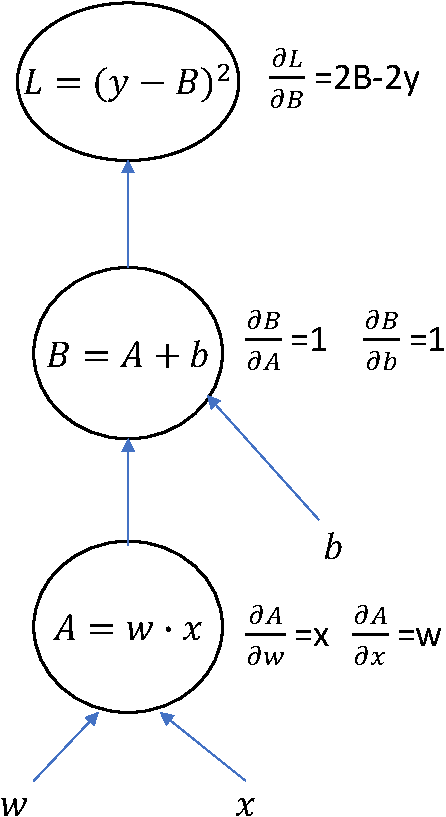
\includegraphics[width=0.25\textwidth]{bp_example.pdf}\\
    Draw the computation graph for equation (\ref{eq:bp2}) including both the forward and backward pass as in the example. Include all the sub-components A-F. At each node, you should include both the sub-component for the forward pass and the gradient for the backward pass. \textit{You may draw on paper or on PowerPoint and use \href{https://www.overleaf.com/learn/latex/Inserting_Images}{includegraphics} to insert the image in LaTex.}
    \textit{Hint: $\frac{\partial \sigma(x)}{\partial x}=\sigma(x)(1-\sigma(x)).$}
\newpage
    
\begin{answertext}{23cm}{}
    
\end{answertext}
\newpage
\item (3 points) Compute the following gradients: $\frac{\partial \mathcal{L}}{\partial \vw_1}$, $\frac{\partial \mathcal{L}}{\partial \vw_2}$, $\frac{\partial \mathcal{L}}{\partial \vx}$. Express your answer in terms of gradients of the sub-components A-F.

\begin{answertext}{6cm}{}
    
\end{answertext}

\item (4 points) Now consider the following initialization:
    \begin{align*}
        \vw_1=\begin{bmatrix}-1 \\ 1\end{bmatrix}\quad\quad
        \vw_2=0.5\quad\quad
        \vx=\begin{bmatrix}1 \\ 2\end{bmatrix}\quad\quad p=0.8
    \end{align*} 
    What are the values of $\vw_1$ and $\vw_2$ after taking one gradient step with learning rate $\eta=0.1$? Show the intermediate value of each node for both the forward (e.g. the value of B) and backward (e.g. the value of $\frac{\partial B}{\partial A}$) pass to ensure partial credit. \textit{Round off your results to three decimal digits.}\\
    \begin{answertext}{11cm}{}
        
    \end{answertext}
\end{enumerate}

\newquestion
\section*{\arabic{QuestionCounter}) Deep Neural Networks (6 points)} 
\begin{enumerate}[(1)]
    \item (2 points) Consider a Convolutional Neural Network applies convolution on a $16\times 16$ feature map, the convolution kernel size is $K=4 \times 4$, stride size $S=2 \times 2$, padding size $P=1 \times 1$. What's the size of the output feature map?\\
    \begin{answertext}{6cm}{}
    
    \end{answertext}

    \item (2 points) What are vanishing gradients and exploding gradients? Which activation function would be more likely to cause the vanishing gradient problem, sigmoid or ReLU? State the reasons.
    
    \begin{answertext}{12cm}{}
        \textbf{Vanishing gradients:} \\\\\\\\\\
        \textbf{Exploding gradients:}\\\\\\\\\\
        \textbf{Sigmoid or ReLU:} \\\\\\\\\\
        \textbf{Reasons:}
    \end{answertext}
    \newpage
    \item (2 points) Explain how auto-encoders can be used for denoising images and feature extraction separately. 
    
    \begin{answertext}{10cm}{}
        \textbf{Denoising images:} \\\\\\\\\\\\\\
        \textbf{Feature extraction:}
    \end{answertext}
\end{enumerate}

\end{document}